%! Author = user
%! Date = 25/01/2021

% Preamble
\documentclass[11pt]{article}

\begin{document}

    \subsection{The Chain of Responsibility Pattern}
    ...
    \begin{itemize}
        \item ...
    \end{itemize}

    \subsection{The Command Pattern}
    This pattern encapsulates a request as an object, thereby letting you parameterize other objects with different
    request, queue or log requests, and support undoable operations.
    \begin{itemize}
        \item This pattern encapsulates a request by binding together a set of actions on a specific reveicer. It packages
        the action and the reveicer up into an object that exposes just one method, execute. When called execute()
        causes the action to be invoked on the receiver.\\
        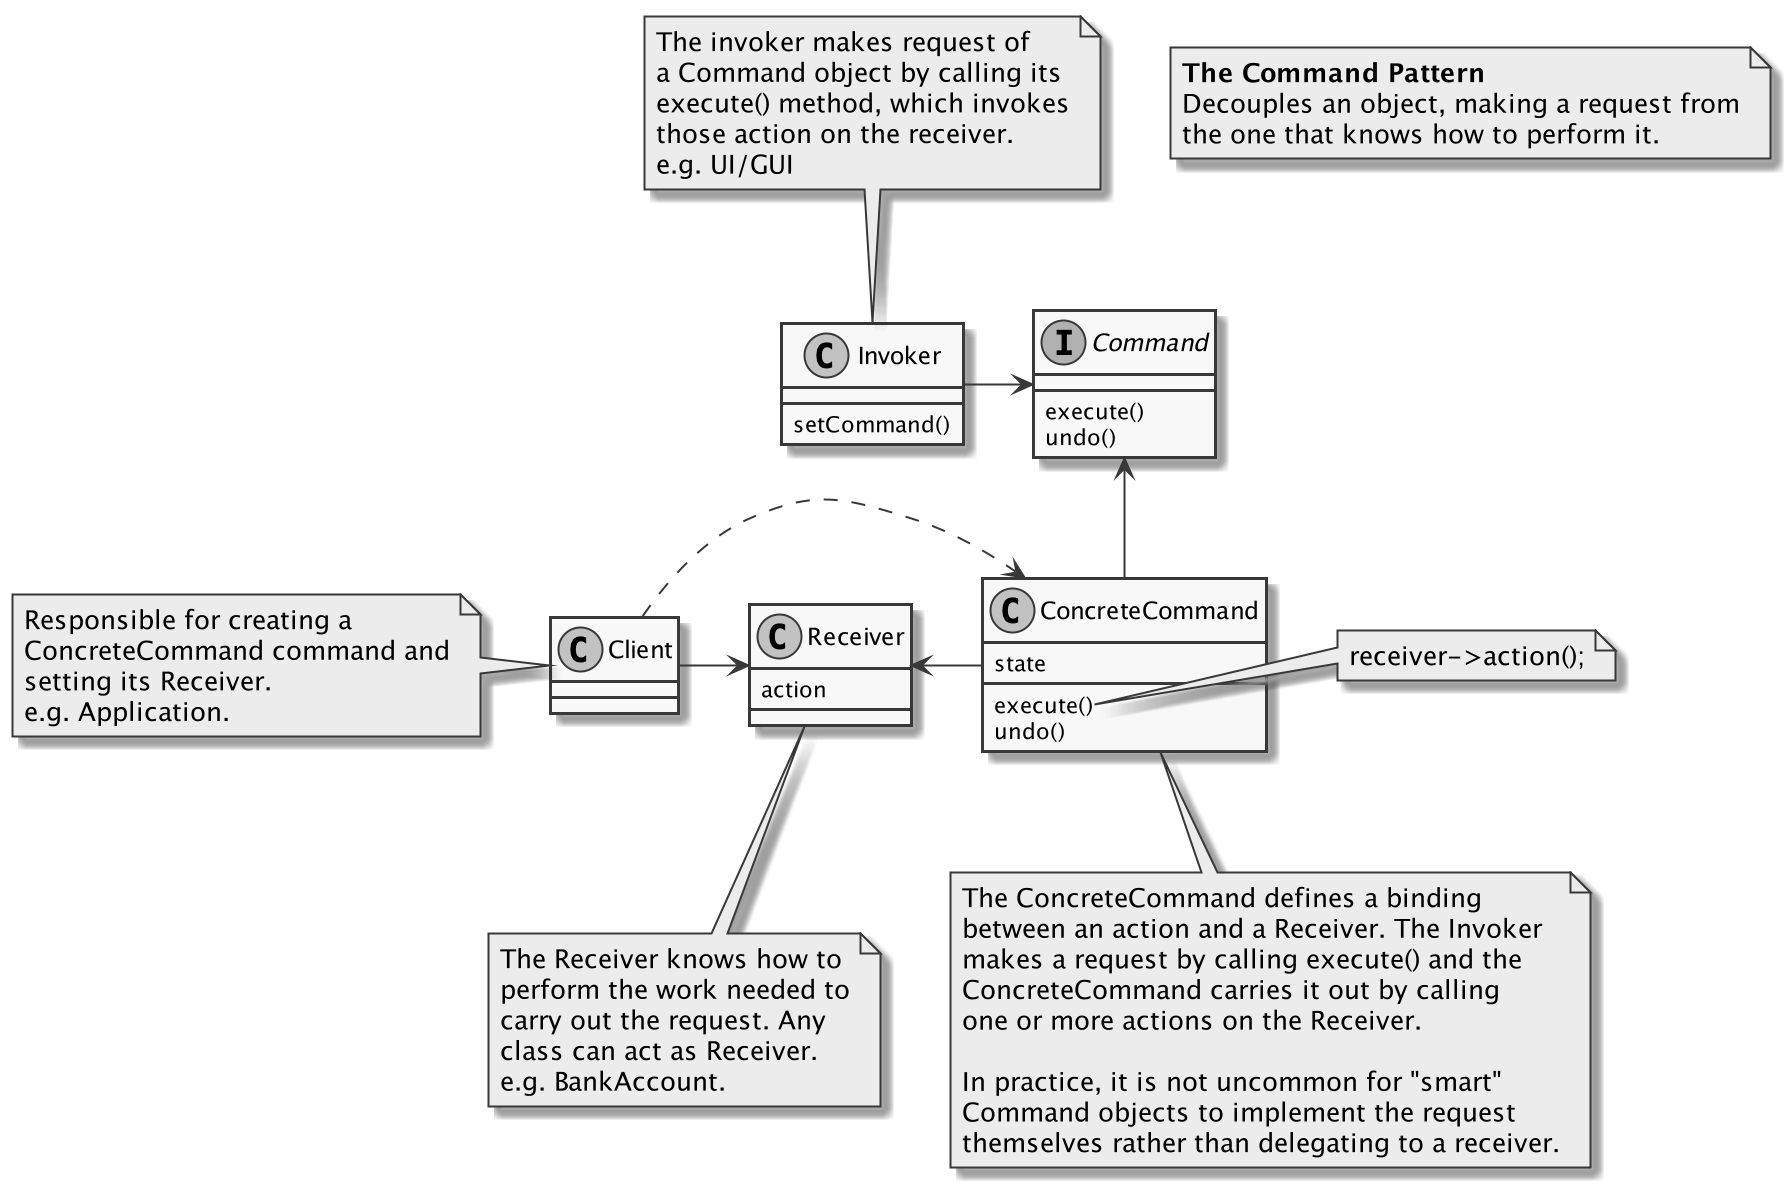
\includegraphics[scale=0.15]{command/1__command}
        \item this pattern:
        \begin{enumerate}
            \item decouples what is done, from who does it
            \item decouples what is done, from when its done
        \end{enumerate}
        \begin{multicols}{2}
            \begin{lstlisting}
class BankAccount {
public:
    BankAccount()
            : balance_(0),
              overdraft_limit_(-500) {
    }

    void Deposit(int amount) {
        balance_ += amount;
    }

    void Withdraw(int amount) {
        if ((balance_ - amount) >= overdraft_limit_) {
            balance_ -= amount;
        }
    }

    int balance_;
    int overdraft_limit_;
};

class ICommand {
public:
    virtual ~ICommand() = default;
    virtual void Execute() const = 0;
    virtual void Undo() const = 0;
};

class Command : ICommand {
public:
    BankAccount &account_;
    int amount_;
    enum Action {
        deposit, withdraw
    } action_;

    Command(BankAccount &account, const Action action, int amount)
            : account_(account),
              amount_(amount),
              action_(action) {
    }

    void Execute() const override {
        switch (action_) {
            case deposit:
                account_.Deposit(amount_);
                break;
            case withdraw:
                account_.Withdraw(amount_);
                break;
            default:
                break;
        }
    }

    void Undo() const override {
        switch (action_) {
            case withdraw:
                account_.Deposit(amount_);
                break;
            case deposit:
                account_.Withdraw(amount_);
                break;
            default:
                break;
        }
    }
};

TEST(command, bankAccount) {
    auto ba = BankAccount();
    EXPECT_EQ(ba.balance_, 0);
    EXPECT_EQ(ba.overdraft_limit_, -500);

    // we have encapsulated everything
    // that needs to be done on the back account.
    std::vector<Command> commands; // list of commands
    commands.emplace_back(Command(ba, Command::deposit, 100));
    commands.emplace_back(Command(ba, Command::withdraw, 200));

    for (auto &c : commands) {
        c.Execute();
    }
    EXPECT_EQ(ba.balance_, -100);
}
            \end{lstlisting}
        \end{multicols}
    \end{itemize}

    \subsection{The Interpreter Pattern}
    ...
    \begin{itemize}
        \item ...
    \end{itemize}

    \subsection{The Iterator Pattern}
    This pattern provides a way to access the elements of an aggregate object sequentially without exposing
    its underlying representation.
    \begin{itemize}
        \item Problem: There are many ways to store objects and data structure e.g. using collection type: array, vector,
        list, linkedlist, set etc.
        \begin{enumerate}
            \item When we have a function that needs to go through the items, the function needs to change if we choose a different
            collection type. e.g. changing from vector to list.
            \item What if we need to write code that operates one several collection types? We need to branch out for
            every collection type.
        \end{enumerate}
        \item The Iterator pattern makes use of the Single Responsibility Principle, and separates the Aggregation
        and the Iteration responsibilities of a collection into two different classes.\\
        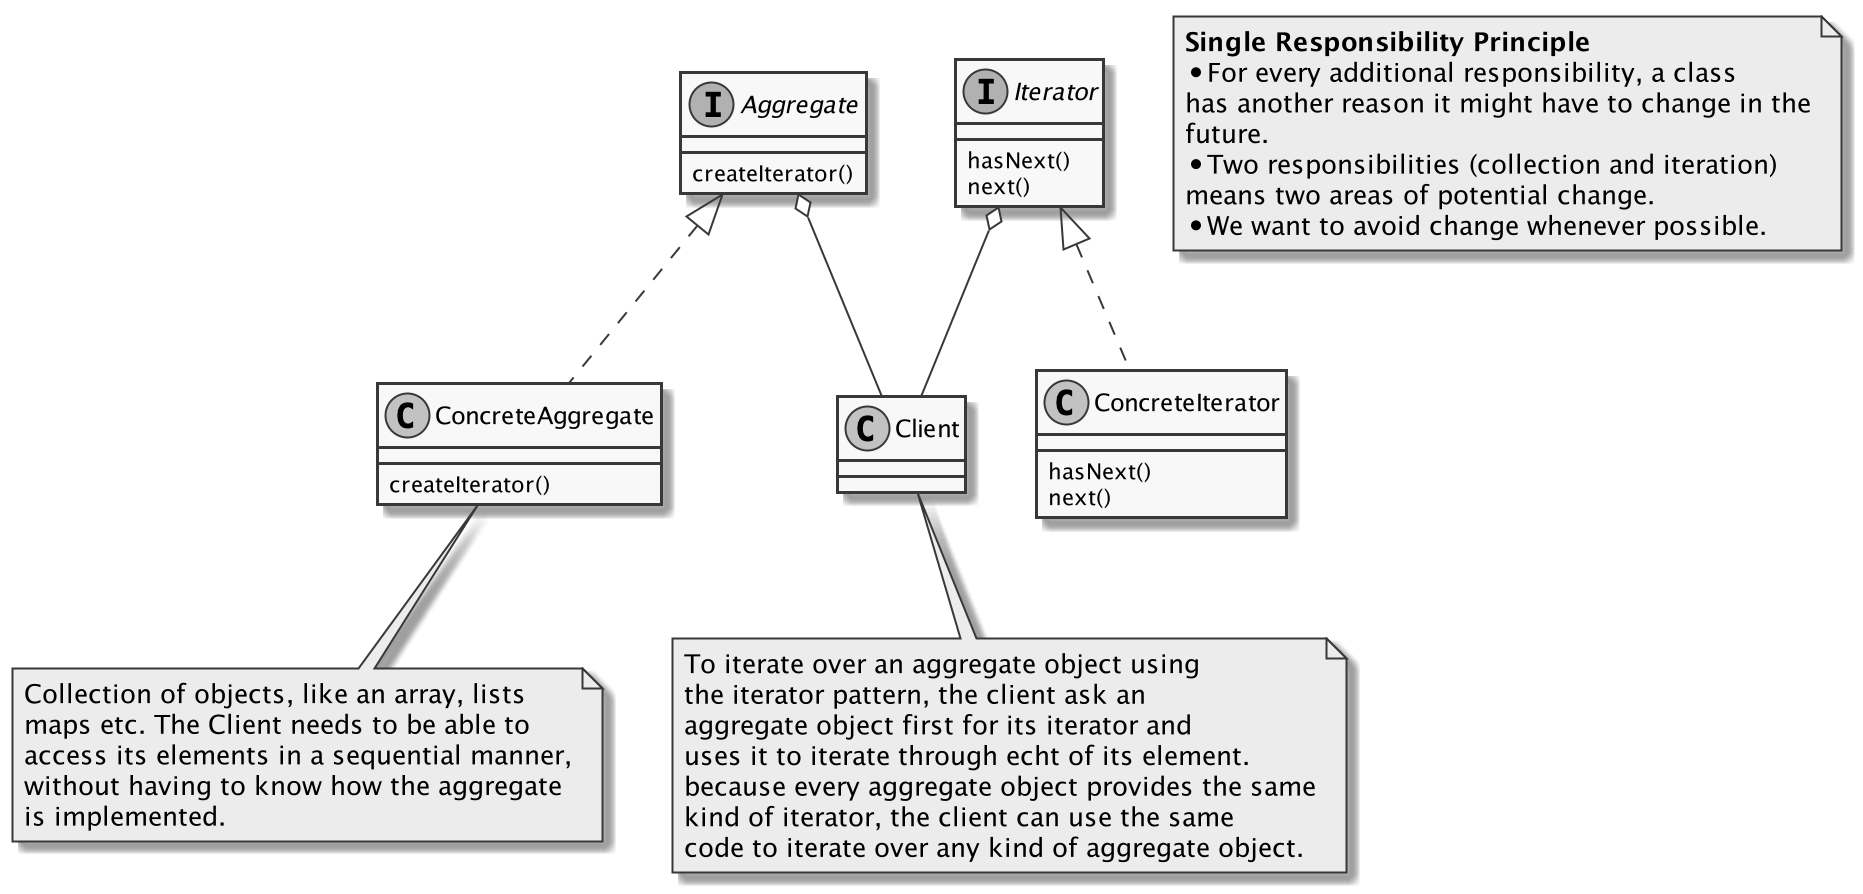
\includegraphics[scale=0.15]{iterator/2__iterator.png}
        \item In C++, Container member functions Requirement:
        \begin{enumerate}
           \item begin() points to first element in the container, if empty, is equal to end();
           \item end() points to the element immediately after the last element.
        \end{enumerate}
        \item In C++, Iterators operators Requirements:
        \begin{enumerate}
            \item operator != must return false if two iterators point to the same element.
            \item operator * (dereferencing) must return a reference to (or a copy of) the data the iterator points to.
            \item operators ++ gets the iterator to point to the next element.
        \end{enumerate}
        \item Example: Binary Tree Iterator:
        \begin{multicols}{2}
            \begin{lstlisting}
template<typename T>
struct BinaryTree;

template<typename T>
struct Node {
    T value = T();
    Node<T> *left = nullptr;
    Node<T> *right = nullptr;
    Node<T> *parent = nullptr;
    BinaryTree<T> *tree = nullptr;

    explicit Node(const T &value)
        : value(value) {
    }

    ~Node() {
        if (left) {
            delete left;
        }
        if (right) {
            delete right;
        }
    }

    Node(const T &value, Node<T> *const left, Node<T> *const right)
        : value(value), left(left), right(right) {
        this->left->tree = this->right->tree = tree;
        this->left->parent = this->right->parent = this;
    }

    void set_tree(BinaryTree<T> *t) {
        tree = t;
        if (left) {
            left->set_tree(t);
        }
        if (right) {
            right->set_tree(t);
        }
    }
};

template<typename T>
struct BinaryTreeIterator {
    Node<T> *current;

    explicit BinaryTreeIterator(Node<T> *const current)
            : current(current) {
    }

    bool operator!=(const BinaryTreeIterator<T> &other) {
        return current != other.current;
    }

    Node<T> &operator*() {
        return *current;
    }

    BinaryTreeIterator<T> &operator++() {
        if (current->right) {
            current = current->right;
            while (current->left) {
                current = current->left;
            }
        } else {
            Node<T> *p = current->parent;
            while (p && current == p->right) {
                current = p;
                p = p->parent;
            }
            current = p;
        }
        return *this;
    }
};

template<typename T>
struct BinaryTree {
    Node<T> *root = nullptr;

    typedef BinaryTreeIterator<T> iterator;

    explicit BinaryTree(Node<T> *const root)
            : root(root) {
        root->set_tree(this);
    }

    ~BinaryTree() {
        if (root) {
            delete root;
        }
    }

    iterator end() {
        return iterator{nullptr};
    }

    iterator begin() {
        Node<T> *n = root;
        if (n) {
            while (n->left) {
                n = n->left;
            }
        }
        return iterator{n};
    }
};

TEST(iterator, tree) {
    BinaryTree<std::string> family{
        new Node<std::string>{"me",
            new Node<std::string>{"mother",
                new Node<std::string>{"grandma"},
                new Node<std::string>{"grandpa"}},
            new Node<std::string>{"father"}
        }
    };

    for (auto it = family.begin(); it != family.end(); ++it) {
        std::cout << (*it).value << std::endl;
    }
}
            \end{lstlisting}
        \end{multicols}
    \end{itemize}

    \subsection{The Mediator Pattern}
    ...
    \begin{itemize}
        \item ...
    \end{itemize}

    \subsection{The Memento Pattern}
    ...
    \begin{itemize}
        \item ...
    \end{itemize}

    \subsection{The Observer Pattern}
    This pattern defines a one-to-many dependency between object so that when one object changes state, all of its
    dependents are notified and updated automatically.
    \begin{itemize}
        \item This pattern exemplifies the loosely coupling design principle. Any changes we make to the subject or the observer
        never affect the other.\\
        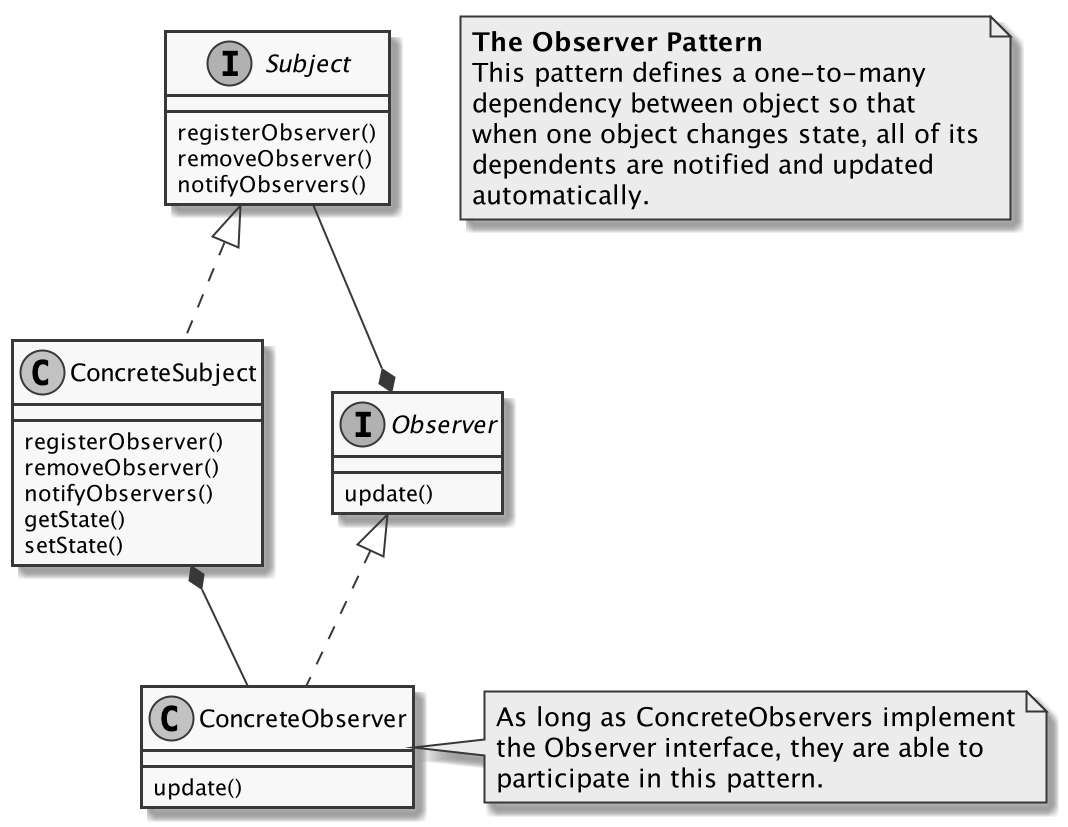
\includegraphics[scale=0.15]{observer/1__loose_coupling}
        \item Subjects and Observers are loosely coupled. They interact, but have little knowledge of each other.
        \begin{enumerate}
            \item Subject knows that the Observer implements a specific interface.
            \item Subject doesn't need to know the concrete class of the Observer.
            \item Observer can be added, removed or replaced at any time. Subject doesn't care; It keeps doing its job.
            \item Any changes made to the Subject or the Observer never affect the other.
        \end{enumerate}
        \item As long as ConcreteObservers implement the Observer interface, they are able to participate in this pattern.
        \item Example:
        \begin{multicols}{2}
            \begin{lstlisting}
class Observer;

class Subject {
public:
    virtual void register(std::shared_ptr<Observer> o) =0;
    virtual void remove(std::shared_ptr<Observer> o) = 0;
    virtual void notify() = 0;
};

class SimpleSubject : public Subject {
public:
    void register(std::shared_ptr<Observer> o) override {
        // add observer to list
        observers_.push_back(o);
    };

    void remove(std::shared_ptr<Observer> o) override {
        // remove observer from list
        observers_.erase(
                std::remove(std::begin(observers_),
                        std::end(observers_), o),
                        std::end(observers_));
    };

    void notify() override {
        std::for_each(std::begin(observers_),
                std::end(observers_),
                [this](auto observer){
            observer->update(value_);
        });
    };

    void setValue(int value){
        value_ = value;
        notify();
    }

private:
    int value_ = 0;
    std::vector<std::shared_ptr<Observer>> observers_;
};

class Observer {
public:
    virtual void update(int value) = 0;
};

class SimpleObserver : public Observer {
public:
    void update(int value) {
        value_ = value;
        std::cout << " updated to " << value_ << std::endl;
    };

    int getValue(){
        return value_;
    }

private:
    int value_ = 0;
};

TEST(observer, observer_example) {
    SimpleSubject simpleSubject;
    auto simpleObserver = std::make_shared<SimpleObserver>();

    simpleSubject.register(simpleObserver);
    simpleSubject.setValue(123);
    EXPECT_EQ(123, simpleObserver->getValue());

    simpleSubject.removeObserver(simpleObserver);
    simpleSubject.setValue(234);
    EXPECT_EQ(123, simpleObserver->getValue());
}
            \end{lstlisting}
        \end{multicols}
    \end{itemize}

    \subsection{The State Pattern}
    ...
    \begin{itemize}
        \item ...
    \end{itemize}

    \subsection{The Strategy Pattern}
    The strategy pattern defines a family of algorithms, encapsulates each one, and makes them interchangable. This lets
    the algorithms vary independent of clients that use them.
    \begin{itemize}
        \item When you overuse inheritance, you can end up with designs that are inflexible and difficult to change. e.g. The Duck simulator\\
        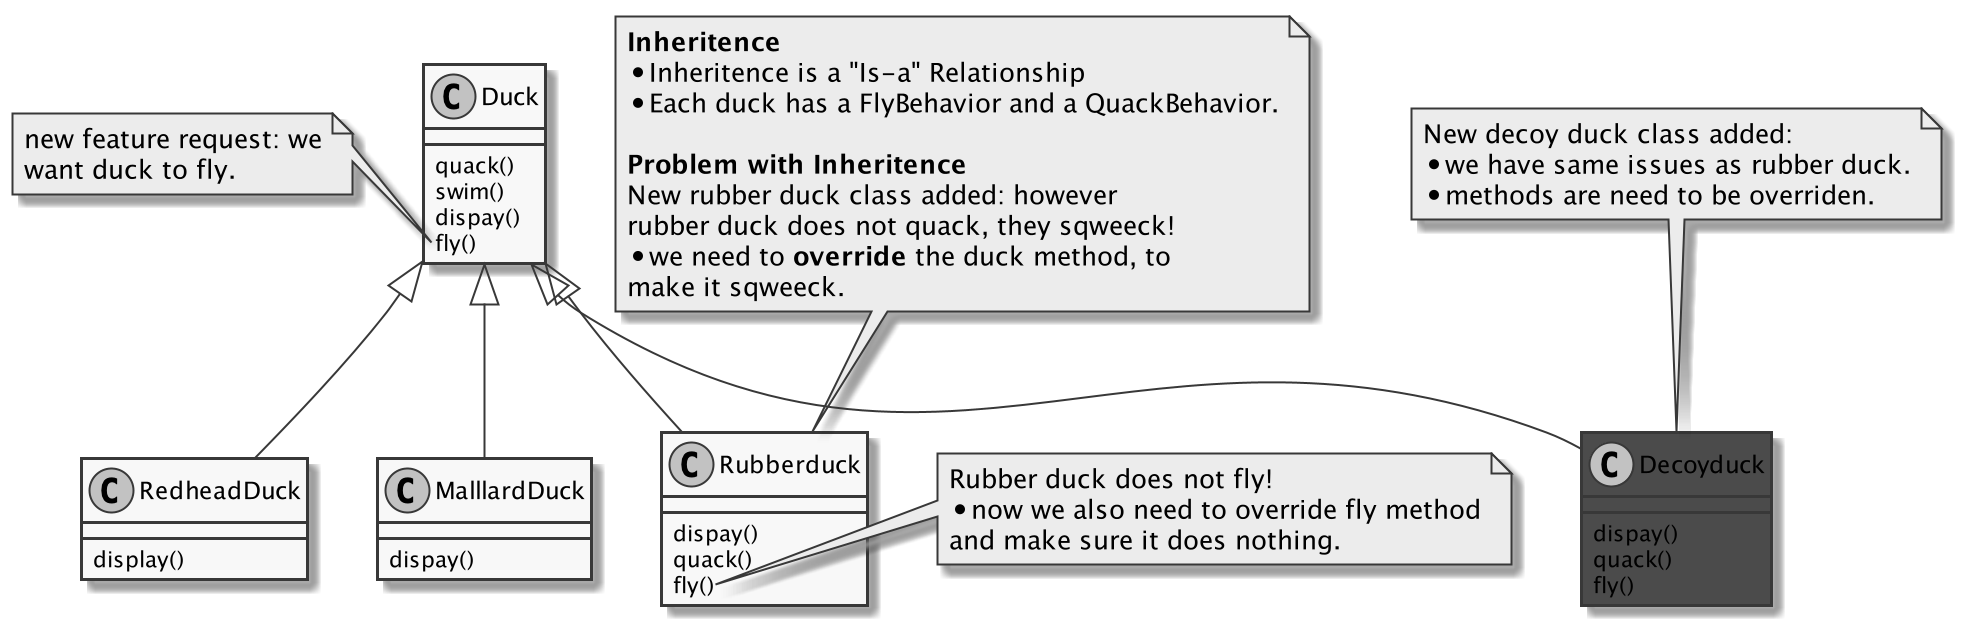
\includegraphics[scale=0.15]{strategy/1_duck_with_hierarchie}
        \item Inheritence doesn't work well here: Behavior changes across subclasses, and its not appropriate for all
        subclasses to have all behaviors. i.e. new rubber duck class added, however rubber duck does not quack, they sqweeck.
        We need to override the duck method, to make it sqweeck.
        \item When using interfaces instead of inheritence. Interfaces defines methods an object must have in order to
        be condisered a particular type.\\
        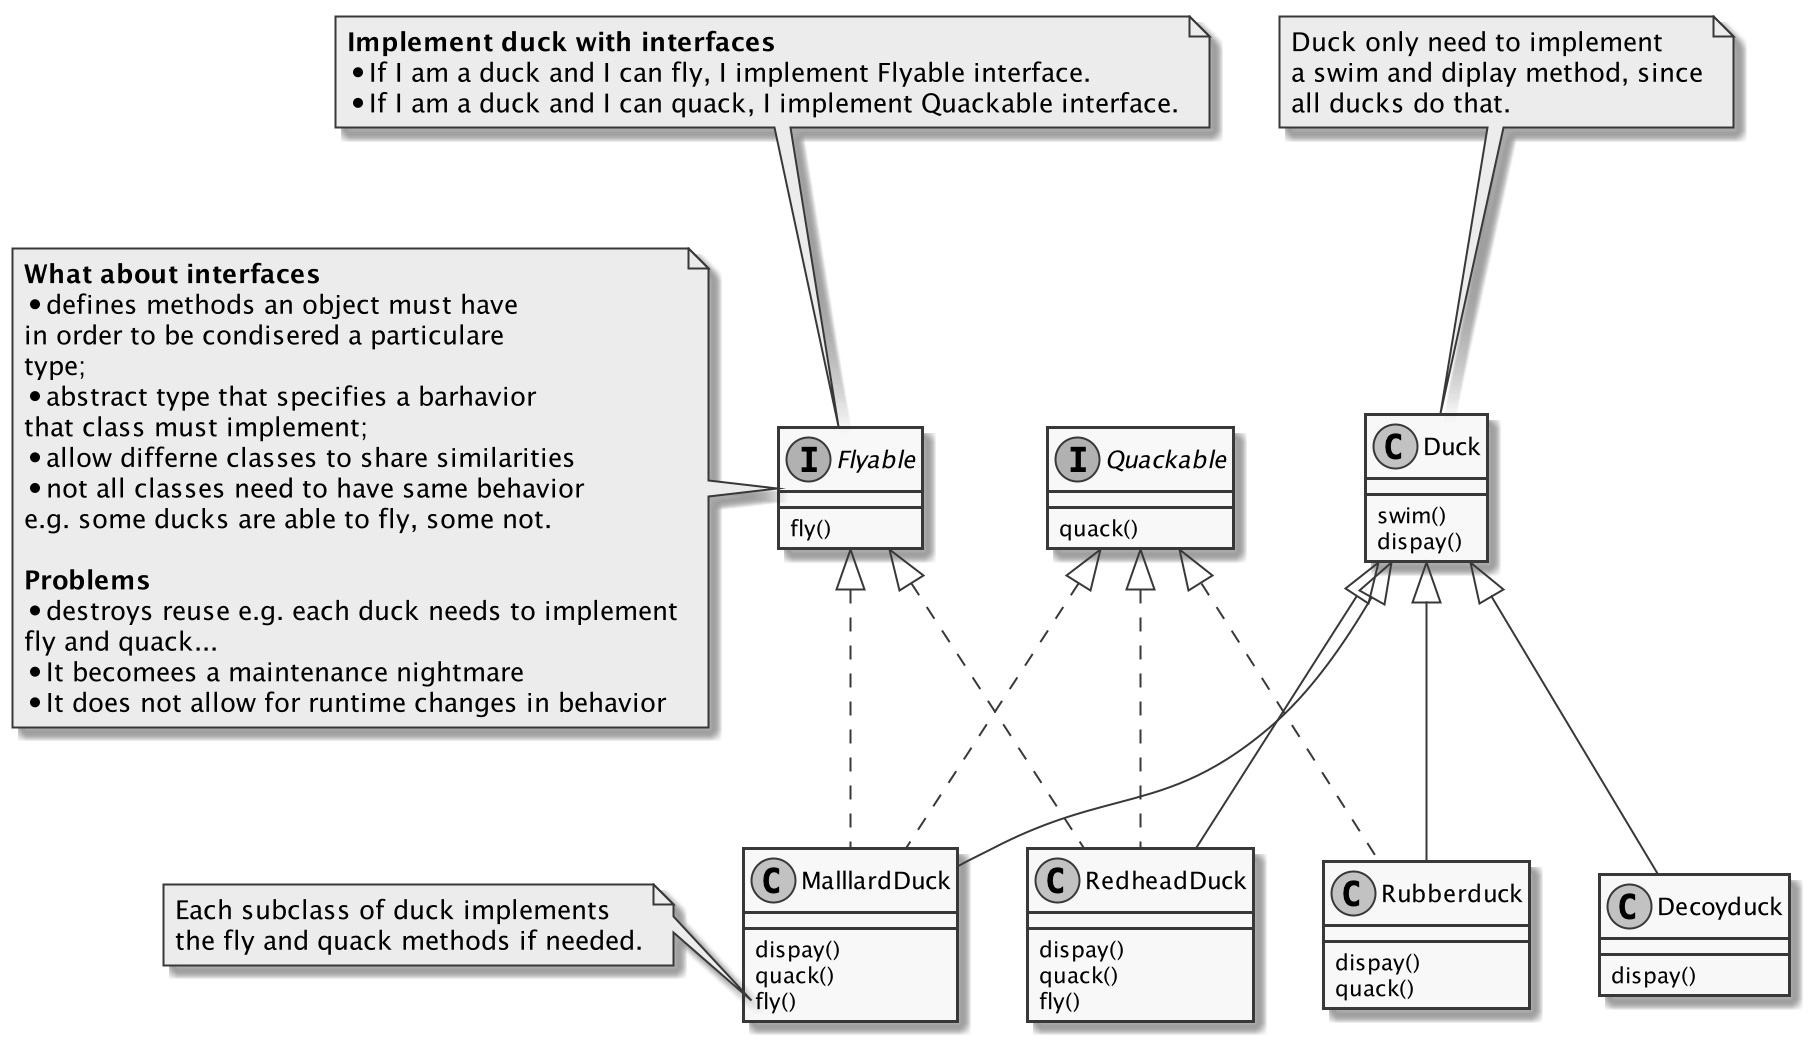
\includegraphics[scale=0.15]{strategy/2_duck_with_interfaces}
        \item Interfaces doesn't work well here: Interfaces supply no implementation and destroys code reuse. This makes
        a maintenance nightmare. i.e. every concrete subclass needs to implement its own flying and quacking behavior.
        \item Strategy make uses of design principles \textbf{encapsulate what varies} and \textbf{program to interface not, implementation}.
        i.e. we pull out varying like the fly() and quack() methods, separate them in a "behavior" classes of which duck
        has reference to. The behavior classes conform to an interface, so we can interchange the behaviors without changing
        the duck.\\
        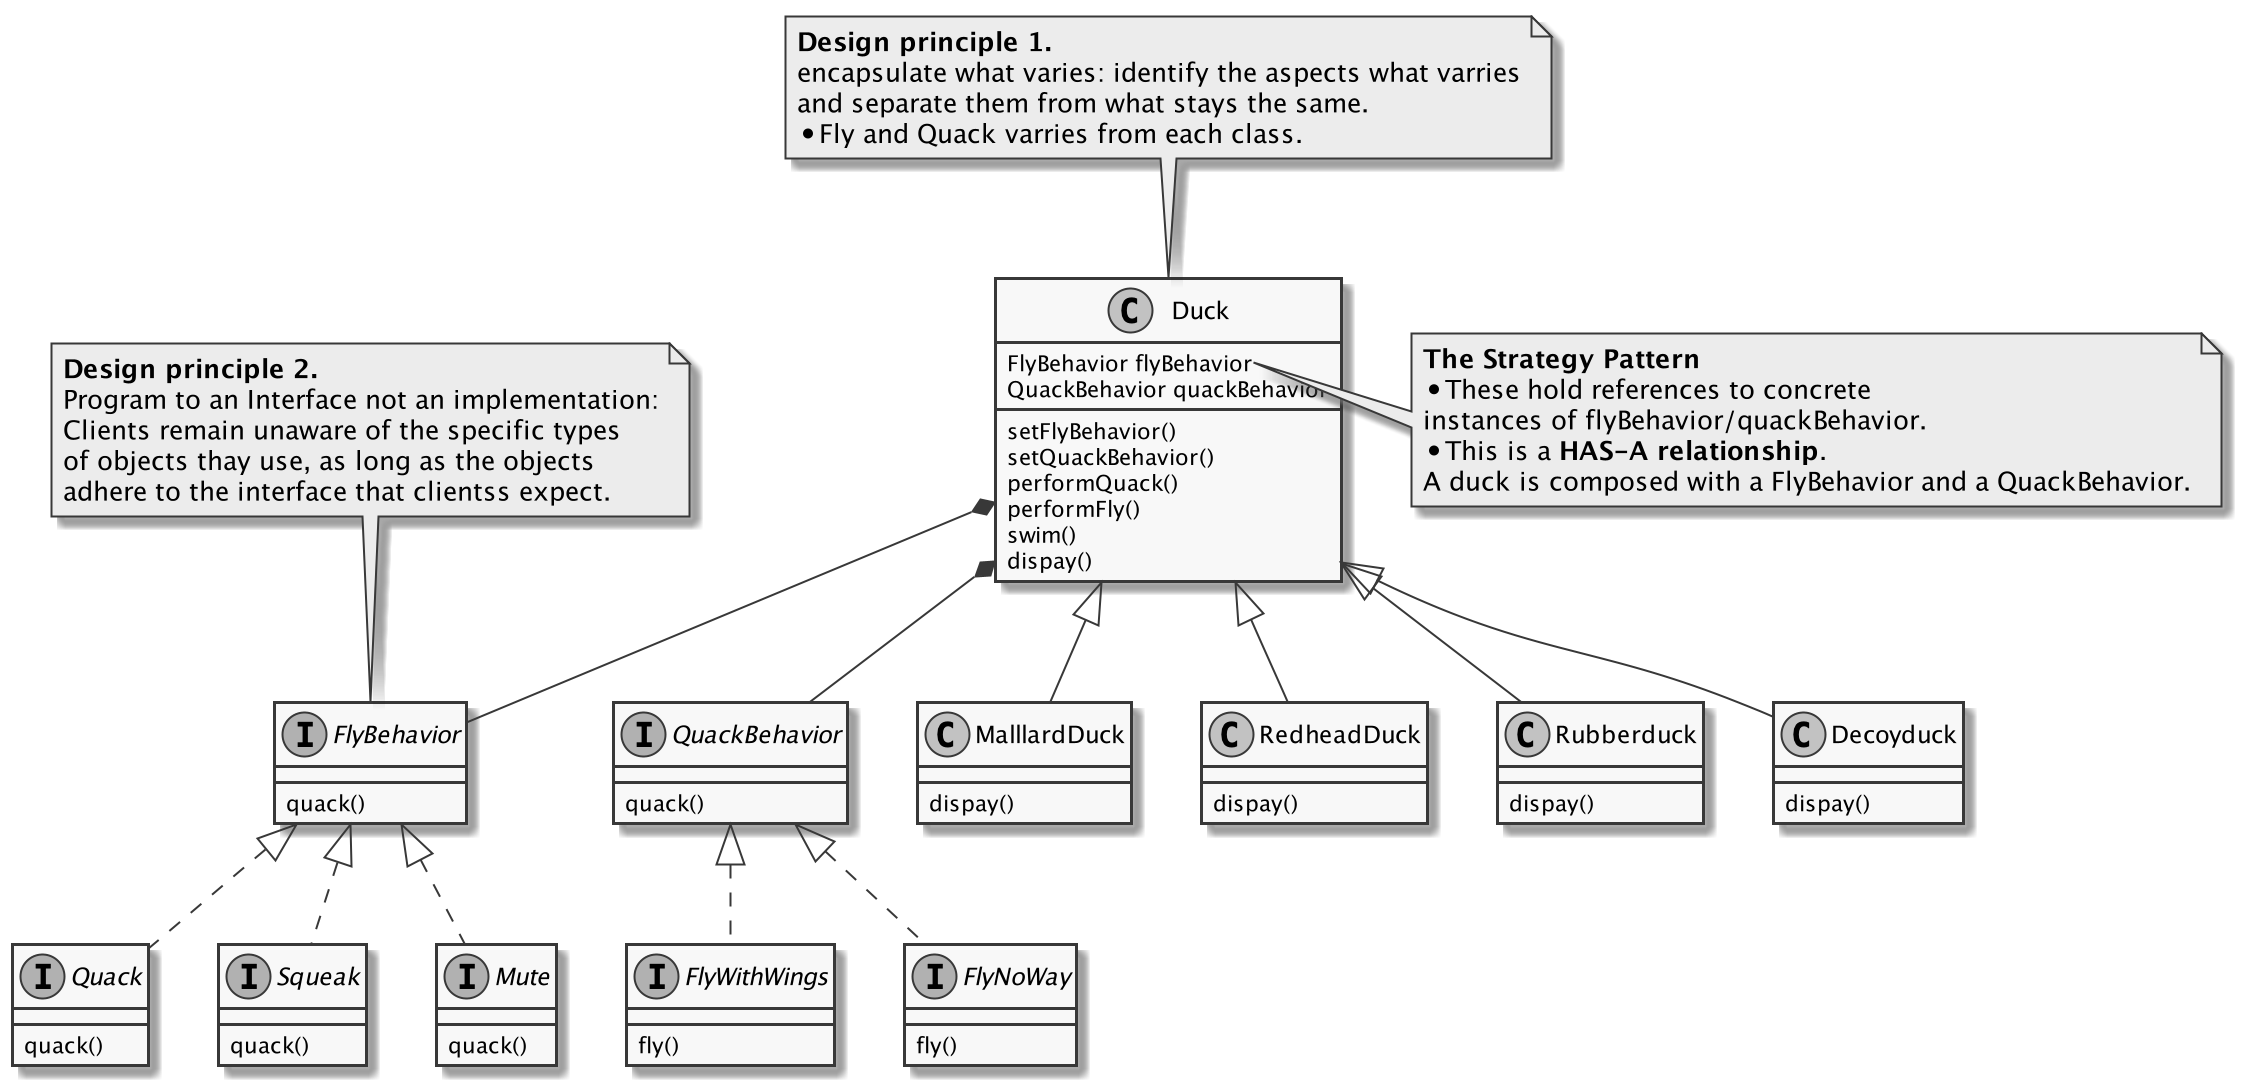
\includegraphics[scale=0.15]{strategy/3_duck_with_interfaces}
        \item Using strategy pattern we have a Has-A relationship between objects and its behaviors. by moving the behaviors
        out of the main inheritance hierarchy, we get the benifit of being able to choose which algorithm each object gets.\\
        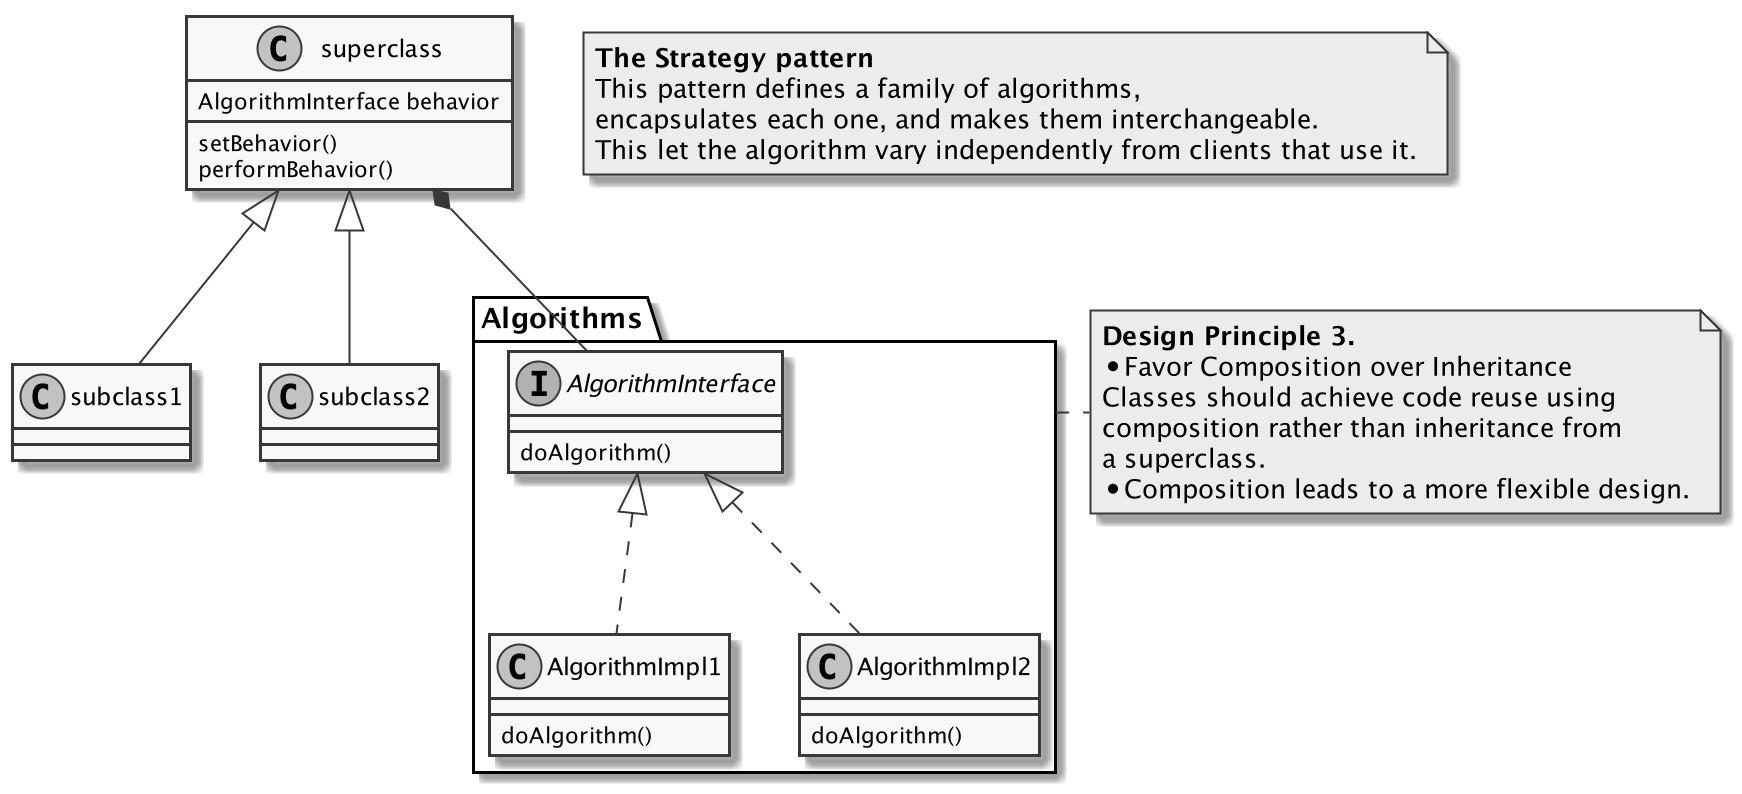
\includegraphics[scale=0.15]{strategy/4_strategy_pattern}
        \item C++ code:
        \begin{multicols}{2}
            \begin{lstlisting}
class FlyBehavior {
public:
    virtual ~FlyBehavior() = default;
    virtual void fly() = 0;
};

class FlyWithWings : public FlyBehavior {
public:
    void fly() override {
        std::cout << "Flap flap!" << std::endl;
    }
};

class FlyNoWay : public FlyBehavior {
public:
    void fly() override {
        std::cout << "I cant fly!" << std::endl;
    }
};

class QuackBehavior {
public:
    virtual ~QuackBehavior() = default;
    virtual void quack() = 0;
};

class Quack : public QuackBehavior {
public:
    void quack() override {
        std::cout << "Quuuuaaaack!" << std::endl;
    }
};

class Mute : public QuackBehavior {
public:
    void quack() override {
        std::cout << "...........!" << std::endl;
    }
};

class Duck {
public:
    Duck(std::unique_ptr<FlyBehavior> fly_behavior, std::unique_ptr<QuackBehavior> quack_behavior)
        : fly_behavior_(move(fly_behavior)), quack_behavior_(move(quack_behavior)){}

    virtual ~Duck() = default;
    void doFly() {
        fly_behavior_->fly();
    };
    void doQuack() {
        quack_behavior_->quack();
    };
    virtual void Display() = 0;

protected:
    std::unique_ptr<FlyBehavior> fly_behavior_;
    std::unique_ptr<QuackBehavior> quack_behavior_;
};

class MallardDuck : public Duck {
public:
    MallardDuck()
            : Duck(std::make_unique<FlyWithWings>(), std::make_unique<Quack>()){}
    MallardDuck(std::unique_ptr<FlyBehavior> fly_behavior, std::unique_ptr<QuackBehavior> quack_behavior)
            : Duck(move(fly_behavior), move(quack_behavior)){}
    void Display() override {
        std::cout << "Display a Mallard Duck" << std::endl;
    };
};

class DecoyDuck : public Duck {
public:
    DecoyDuck()
            : Duck(std::make_unique<FlyNoWay>(), std::make_unique<Mute>()){}
    void Display() override {
        std::cout << "Display a Decoy Duck" << std::endl;
    };
};

TEST(strategy, duck) {
    MallardDuck mallerd;
    DecoyDuck decoy;

    std::vector<Duck*> ducks;
    ducks.push_back(&mallerd);
    ducks.push_back(&decoy);

    for(auto& duck: ducks){
        duck->doFly();
        duck->doQuack();
        duck->Display();
    }
}
            \end{lstlisting}
        \end{multicols}
    \end{itemize}

    \subsection{The Template Method Pattern}
    ...
    \begin{itemize}
        \item ...
    \end{itemize}

    \subsection{The Visitor Pattern}
    ...
    \begin{itemize}
        \item ...
    \end{itemize}

\end{document}
